\section{Measuring parametrization effects}
\label{sec:parametrizing}

After implementing the \ac{pimc} search previously described, some tests were executed in order to observe the effects of different parametrizations.
These tests had to be comparative and a baseline or benchmark was required to establish a standard measure.


\subsection{Creating benchmarks}
The baseline agent was called Rule-based and its main idea was to choose a move considering predefined rules, instead of using hard computational algorithms.
It tries to roughly reproduce the reasoning of a non-professional human player.
%The following pseudo-code illustrates the deliberation process of this agent and tries to roughly reproduce the reasoning of a non-professional human player.

Its procedure starts by collecting the highest cards of each allowed suit for the current play.
The possibility of playing such a highest card is granted by two requirements: being the highest unplayed card of that suit; and not holding at least other 5 cards from that suit, except for the trump suit.
Otherwise, this rule-based player return the lowest possible card.

The first experiments to test this baseline player compare three different scenarios:
\begin{itemize}
\item (a) 1000 games with 4 Rule-based players [dark green];
\item (b) 1000 games with 1 Rule-based player and 3 Random players [red];
\item (c) 1000 games with 2 Rule-based players against 2 Random players [dark blue].
\end{itemize}
Each scenario has a corresponding colour that will be used in every chart for the same scenario.

\begin{figure}[h]
        \centering
        \begin{subfigure}[h]{0.32\textwidth}
                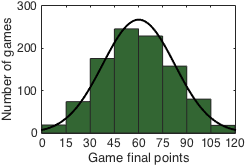
\includegraphics[width=\textwidth]{./img/4/histA}
                \caption{Scenario A}
                \label{fig:histA}
        \end{subfigure}
        \begin{subfigure}[h]{0.32\textwidth}
                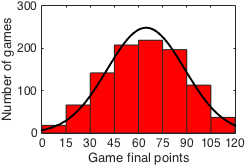
\includegraphics[width=\textwidth]{./img/4/histB}
                \caption{Scenario B}
                \label{fig:histB}
        \end{subfigure}
        \begin{subfigure}[h]{0.32\textwidth}
                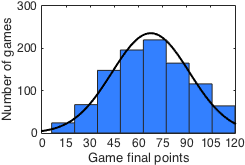
\includegraphics[width=\textwidth]{./img/4/histC}
                \caption{Scenario C}
                \label{fig:histC}
        \end{subfigure}
        \caption[Histograms of the final points obtained in the 3 scenarios]{Histograms of the final points obtained in 1000 games by: (a) one of the teams; (b) the team with 1 Rule-based player and 1 Random player; (c) the team with 2 Rule-based players}
        \label{fig:histograms}
\end{figure}

The histograms presented on Figure~\ref{fig:histograms} exhibit the distribution of final points in 1000 games by one of the teams in each scenario.
However, comparing the three histograms gets easier when merging the three fitting curves in one graph, Figure~\ref{fig:ABC}.

\begin{figure}[h!]
  \centering
    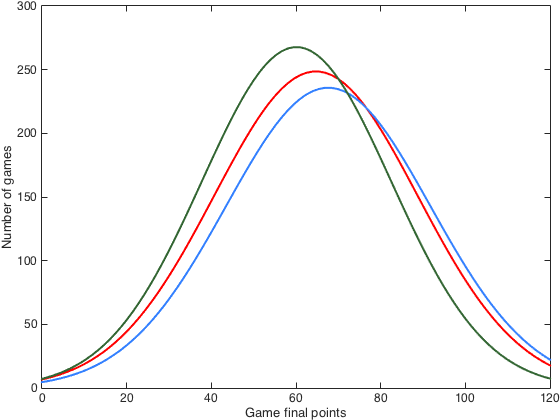
\includegraphics[width=0.5\textwidth]{./img/4/ABC}
  \caption{Fitting curves of histograms presented on Figure~\ref{fig:histograms} with the same colour scheme}
\label{fig:ABC}
\end{figure}

In scenario (a), results were very balanced, as expected, because all players had the same deliberation process.
In 1000 games, one of the teams obtained a winning percentage of 48.5\%, a drawing percentage of 1.9\% and a losing percentage of 49.6\%.
The scenario (b) showed that a team with 1 Rule-based player and 1 Random player can beat a 2 Random players team with a winning percentage of 51.6\%, a drawing percentage of 1.8\% and a losing percentage of 41.6\%.
Finally, in scenario (c), the team with 2 Rule-based players beat the the 2 Random players with the highest winning percentage of 61.1\%, a drawing percentage of 1.8\% and losing percentage of 37.1\%.

A player's performance can only be measured when playing with different players; otherwise, playing a considerable amount of games will balance the winning and losing rates, as seen in scenario (a).
Additionally, theses results also demonstrated the impact of the team player on the team score, since having 2 Rule-based players in the same team increased the winning rate of the team with only 1 Rule-based player.

%In addition to these conclusions, the winning rates achieved by 1 Rule-based (scenario (b)) and 2 Rule-based (scenario (c)) were lower than expected, since their opponents have completely random procedures for playing the game.
In addition to these conclusions, considering the opponents of both teams in scenarios (b) and (c) have completely random procedures for playing the game, their winning rates were expected to be lower.
A possible reason might be \emph{Sueca}'s element of chance, which means certain hands can limit the result even though the opponents are Random players.

This idea incited some research on the influence of the players' initial conditions on the game result.
On the one hand, the power of a hand is completely dependent on the playing style of each player, and therefore, using Random players to measure this property is inappropriate.
On the other hand, this measure will not be used to carefully predict a hand's effect on the final result.
Instead, its goal is to generally classify a hand in one out of three distinct categories (\emph{hard}, \emph{medium} and \emph{easy}) and to filter the hands that are hardly or easily capable of winning.
As a result, the chosen scenario to extract these categories' features was (a).

In order to derive such characteristics, the first step is to speculate and collect possible features of the initial game conditions that may influence the final result.
The next step is computing a linear regression on that data to decide the relevant features.
In the first iterations of this process, many variables were tested for one player of the team and also for both.
For instance, the total points, the trump points, the number of aces, the number of sevens, the number of trumps, being the first to play, having the trump ace, the number of suits.
However, many of them were rejected by the null hypothesis with a significance level of 0.05, and the remaining features were only three: team aces number, team sevens number and team trumps number.

\begin{figure}[h!]
  \centering
    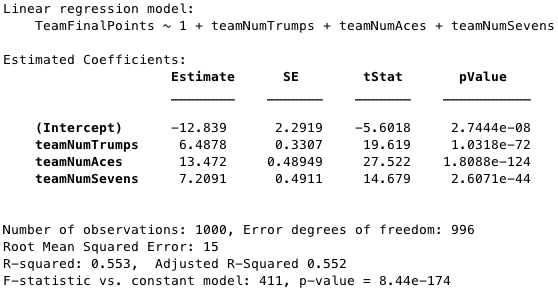
\includegraphics[width=0.7\textwidth]{./img/4/linearRegression}
  \caption{Linear regression with the \emph{team aces number}, the \emph{team sevens number} and the \emph{team trumps number} as predictor variables and \emph{team final points} as the response variable}
\label{fig:linearRegression}
\end{figure}

Figure~\ref{fig:linearRegression} shows the detailed statistic relationship of the mentioned variables on the team final result.
Although the model has a low r-squared value, the p-values of the predictors can reject their null hypothesis and prove their importance in the final result.

\begin{figure}[h]
        \centering
        \begin{subfigure}[h]{0.32\textwidth}
                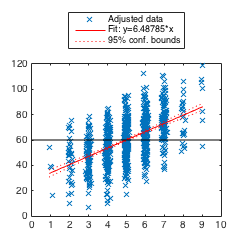
\includegraphics[width=\textwidth]{./img/4/teamTrumpsNumber}
                \caption{Variable \emph{team trumps number}}
                \label{fig:teamTrumpsNumber}
        \end{subfigure}
        \begin{subfigure}[h]{0.32\textwidth}
                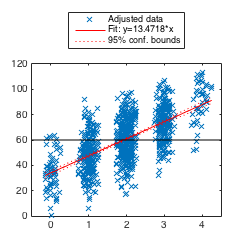
\includegraphics[width=\textwidth]{./img/4/teamAcesNumber}
                \caption{Variable \emph{team aces number}}
                \label{fig:teamAcesNumber}
        \end{subfigure}
        \begin{subfigure}[h]{0.32\textwidth}
                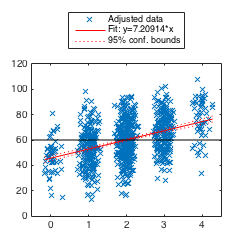
\includegraphics[width=\textwidth]{./img/4/teamSevensNumber}
                \caption{Variable \emph{team sevens number}}
                \label{fig:teamSevensNumber}
        \end{subfigure}
        \caption{Fitting function for each individual predictor variable}
        \label{fig:fitFunctions}
\end{figure}

Finally, Figure~\ref{fig:fitFunctions} can help quantifying the importance of each feature and to build the domain values for each class (\emph{hard}, \emph{medium} and \emph{low}).
Regarding the Figure~\ref{fig:teamTrumpsNumber}, the numbers of initial trumps held by a team, where at least 60\% of the samples were lost games, are 1, 2, 3 and 4.
In the same way, the numbers of initial trumps held by a team, where ate least 60\% of the samples were won games, are 6, 7, 8 and 9.
Applying the same procedure to the three predictor variables, the decided \emph{hard} initial conditions to a team (with low probability of winning) are having at most 4 trumps, at most 1 ace and at most 1 seven.
Conversely, the decided \emph{easy} initial conditions to a team (with high probability of winning) are to have at least 6 trumps, at least 3 aces and at least 3 sevens.
Other cases are considered \emph{medium} hands.

The developed classifications will be used in two different measures: (1) the \ac{fgr}, which means the percentage of won or drawn games; (2) the histogram of points obtained by a certain team.
The first measure is more general and is used to compare the effective performance of players.
On the other hand, the second measure details the points distribution, since the same \acp{fgr} can lead to a different histogram of the final points.

\begin{figure}[h]
        \centering
        \begin{subfigure}[h]{0.32\textwidth}
                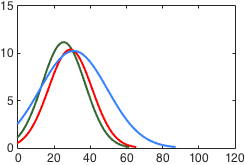
\includegraphics[width=\textwidth]{./img/4/ABChard}
                \caption{filipa}
                \label{fig:ABC-Hhard}
        \end{subfigure}
        \begin{subfigure}[h]{0.32\textwidth}
                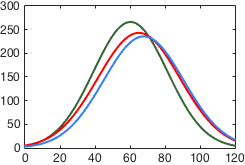
\includegraphics[width=\textwidth]{./img/4/ABCmedium}
                \caption{filipa}
                \label{fig:ABC-Hmedium}
        \end{subfigure}
        \begin{subfigure}[h]{0.32\textwidth}
                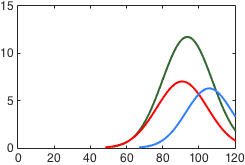
\includegraphics[width=\textwidth]{./img/4/ABCeasy}
                \caption{filipa}
                \label{fig:ABC-Heasy}
        \end{subfigure}
        \caption{filipa}
        \label{fig:ABC-CH}
\end{figure}

Figure~\ref{fig:ABC-CH} shows the distribution of the final points obtained in scenarios (a), (b) and (c) divided into the three aforementioned classifications.
The goal of dividing Figure~\ref{fig:fitHistABC} is to see if the detected differences play a prominent role in each individual initial hand type.
However, out of each 1000 collected games, a few percentage refers to games with \emph{hard} or \emph{easy} initial conditions (between 2\% and 3\% each one), which means the apparent results from \emph{hard} and \emph{easy} initial conditions have low confidence values.
The final points of a team are higher as its Gaussian fitting curve moves to the right in the x axe.
Hence, the distribution charts for \emph{hard} and \emph{medium} evidence the same results: the team with 1 Rule-based player (b) achieved higher final scores and the team with 2 Ruled-based players (c) obtained even higher when compared to 4 Random players (a).
Nevertheless, regarding \emph{easy} initial conditions, the team with 1 Rule-based player underperforms slightly the other two scenarios.

\begin{figure}[h!]
  \centering
    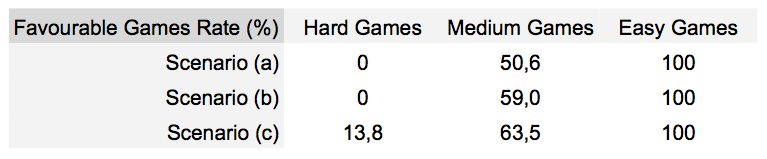
\includegraphics[width=0.7\textwidth]{./img/4/ABC-fgr}
  \caption{filipa}
\label{fig:ABC-fgr}
\end{figure}

Additionally, the \acp{fgr}, presented in Figure~\ref{fig:ABC-fgr}, measure the effectiveness of players when competing with each other.
This rate also evidenced that the Rule-based player outperforms the Random player, mainly based on the \ac{fgr} of the \emph{medium} hands, in which the confidence is higher due to number of samples.

In sum, the Rule-based player guided the development of new measures and will be the benchmark for evaluating the \ac{pimc} algorithm.


\subsection{The Trick Player}

The \ac{pimc} algorithm, implemented as described in Section~\ref{sec:implementing}, cannot explore complete trees until the middle of the game, and therefore, the depth had to be limited.
So, the first two possible parametrizations of the algorithm were the depth limit and the \emph{N} that defines the number of different distributions to be sampled while choosing a card to play.
As a result, two distinct branches were clear, creating a version with a low depth limit and a high \emph{N} value, and another one that has a higher depth limit with lower \emph{N} values.
Additionally, the third possible parametrization is the utility function used by the player.

The Trick player, as the name suggests, evaluates only one trick of every game tree (depth limit of 1) and samples 1000 different distributions (\emph{N} value).
The mean time of its deliberation process for each move is 0.13 seconds.
Its utility function is modelled by:
\begin{equation} \label{eq:uf1}
u_1 = \left\{
                \begin{array}{ll}
                  teamPoints, & teamPoints \geq opponentTeamPoints\\
                  - opponentTeamPoints, & teamPoints < opponentTeamPoints
                \end{array}
              \right.
\end{equation}

In order to observe the Trick player performance, the following scenarios will be considered:
\begin{itemize}
\item (d) 1000 games with 1 Trick player and 3 Rule-based players [yellow];
\item (e) 1000 games with 2 Trick players against 2 Rule-based players [orange].
\end{itemize}

The \ac{fgr} of the team with 1 Trick player and 1 Rule-based (d) was 52.8\% (50.5\% won games and 2.3\% drawn games), and at the same time, the \ac{fgr} of the team with 2 Trick players (e) was 55.6\% (53.4\% won games and 2.2\% drawn games).
In the same way there was a difference between scenarios (b) and (c), having two Trick players on the same team significantly improves the results when compared to only one.
This evidence was expected, since \emph{Sueca} is a team game.

\begin{figure}[h!]
  \centering
    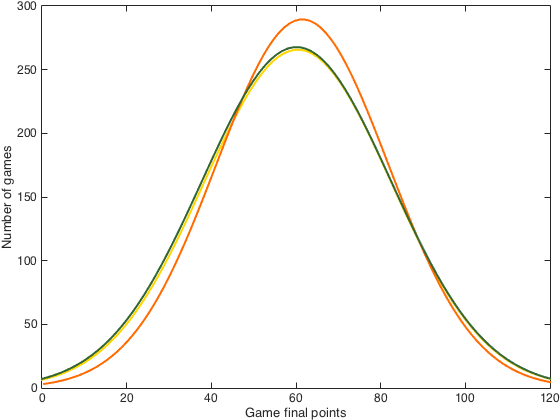
\includegraphics[width=0.5\textwidth]{./img/4/ADE}
  \caption{filipa}
\label{fig:ADE}
\end{figure}

Additionally, Figure~\ref{fig:ADE} presents the distributions of the 1000 obtained final scores from each scenario.
Scenario (a, green) was also included to provide a baseline of equilibrium.
The Gaussian fitting curve of scenario (d, yellow) is nearly coincident with the one of scenario (a), suggesting one Trick player in a team does not influence the results.
On the other hand, a team with 2 Trick players, scenario (e, orange), evidences a higher distribution between 60 and 80 points.
These conclusions are also supported by the \acp{fgr} of 50.4\%, 50.5\% and 53.4\% from the teams of scenarios (a), (d) and (e), respectively.

\begin{figure}[h]
        \centering
        \begin{subfigure}[h]{0.32\textwidth}
                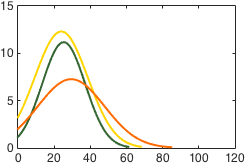
\includegraphics[width=\textwidth]{./img/4/ADEhard}
                \caption{filipa}
                \label{fig:ADEhard}
        \end{subfigure}
        \begin{subfigure}[h]{0.32\textwidth}
                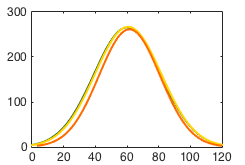
\includegraphics[width=\textwidth]{./img/4/ADEmedium}
                \caption{filipa}
                \label{fig:ADEmedium}
        \end{subfigure}
        \begin{subfigure}[h]{0.32\textwidth}
                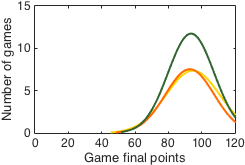
\includegraphics[width=\textwidth]{./img/4/ADEeasy}
                \caption{filipa}
                \label{fig:ADEeasy}
        \end{subfigure}
        \caption{filipa}
        \label{fig:ADE-CH}
\end{figure}

When analysing the Gaussian fitting curves divided into the classes of initial hands, results agree with previous conclusions, except for the \emph{hard} classification of initial conditions.
So, in scenario (e, orange) the team of 2 Trick players achieved higher scores with \emph{hard} and \emph{medium} hands, while with \emph{easy} hands the modal values of the three scenarios seem to be concurrent.
However, as previously mentioned, out of each 1000 collected games, a few percentage refers to games with \emph{hard} or \emph{easy} initial conditions (between 2\% and 3\% each one), which means the apparent results from \emph{hard} and \emph{easy} initial conditions have low confidence values.

\begin{figure}[h!]
  \centering
    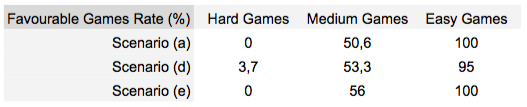
\includegraphics[width=0.7\textwidth]{./img/4/ADE-fgr}
  \caption{filipa}
\label{fig:ADE-fgr}
\end{figure}

Moreover, the \acp{fgr} in Figure~\ref{fig:ADE-fgr} evidenced that the Trick player slightly outperforms the Rule-based player, mainly based on the \ac{fgr} of the \emph{medium} hands, in which the confidence is higher due to number of samples.
The unexpected differences on scenario (d) with both \emph{hard} and \emph{easy} initial conditions refer to only one game, in both cases, and may reflect some flaws on the classification inferred from the linear regression.



\subsection{The Deep-1 Player}

In contrast to the last player, which has a low depth limit and high \emph{N} value, the Deep-1 player has the highest reasonable depth limit and lower \emph{N} values.
In other words, each time this player has to choose a move, it sets the maximum depth limit considering it has to sample at least 30 different distributions and its deliberation time must be less than 2 seconds.
Figure~\ref{fig:nDepthLimits} shows the chosen \emph{N} values and depth limits for each tree size, and also the explored depth percentage.

\begin{figure}[h!]
  \centering
    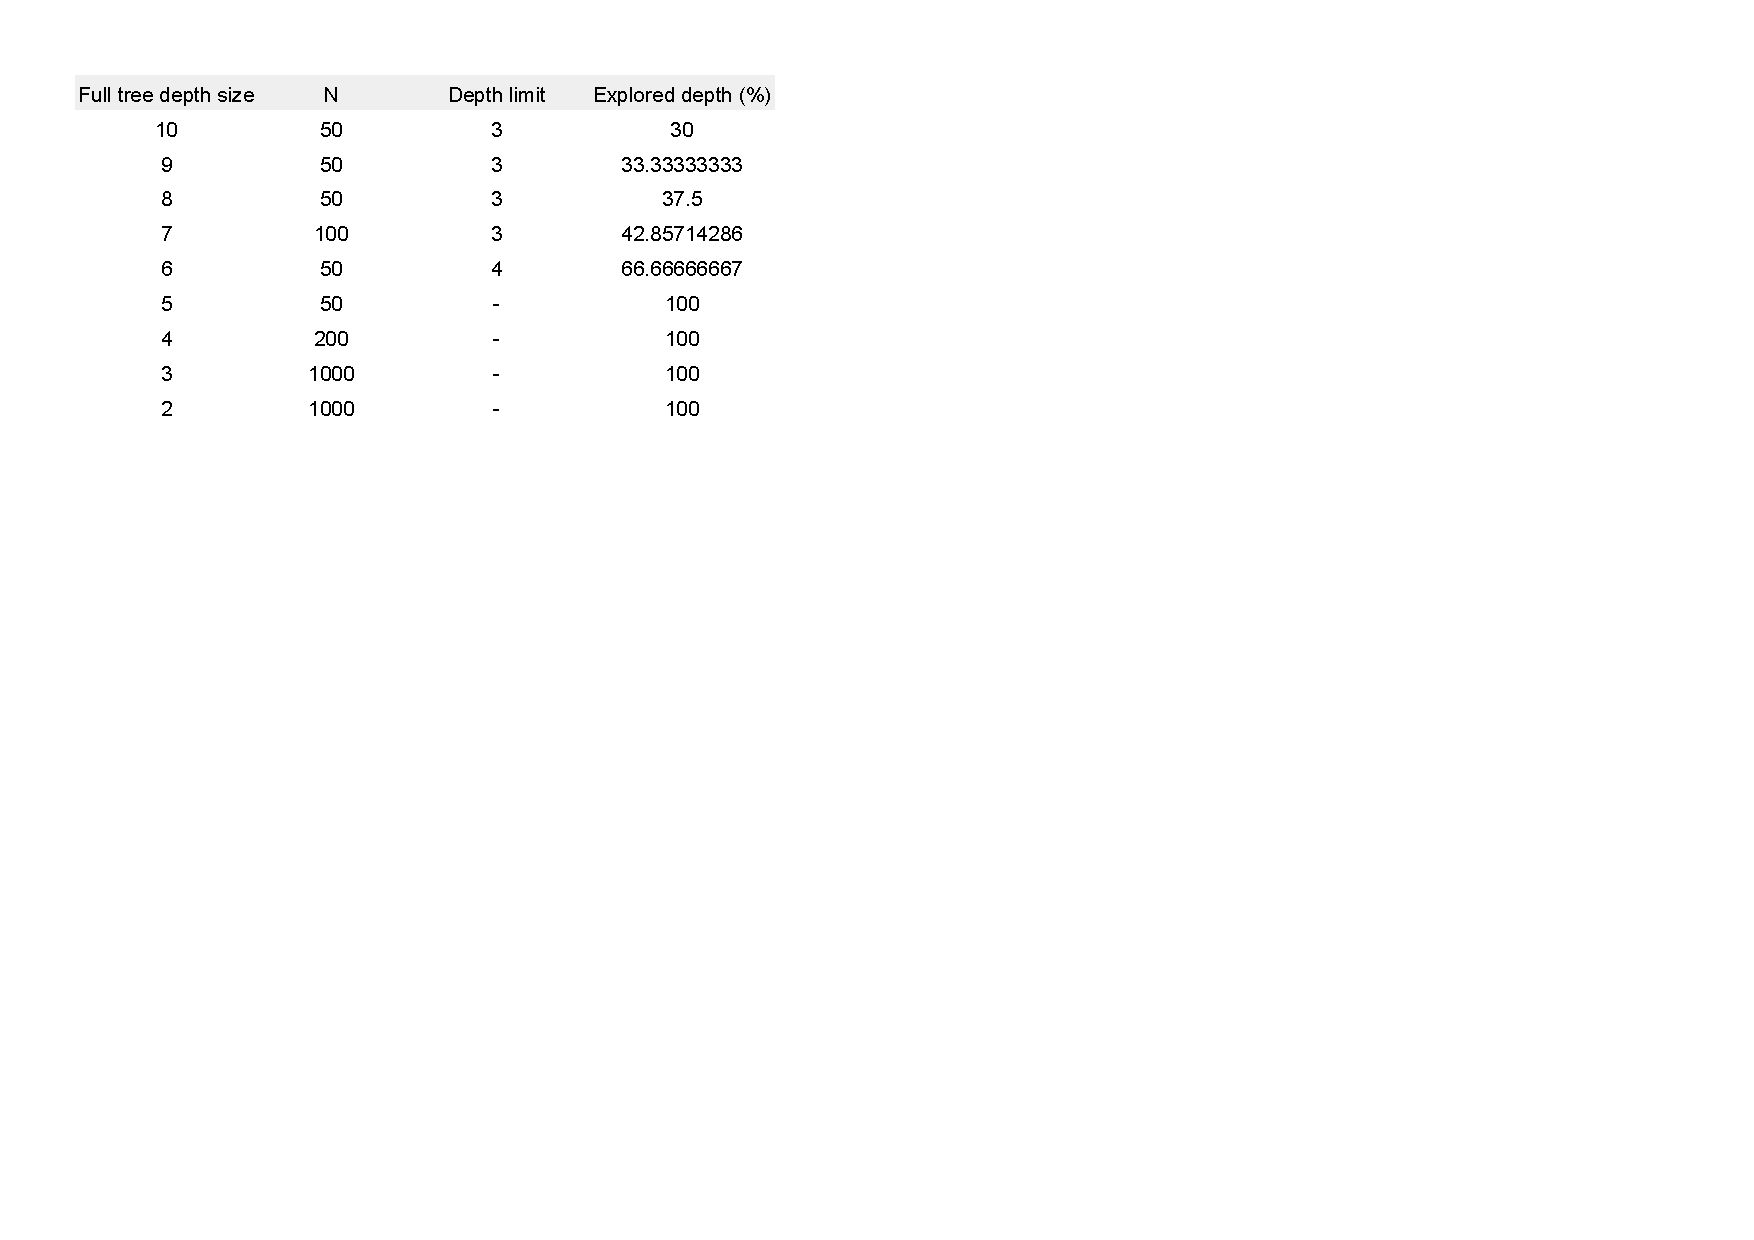
\includegraphics[width=0.7\textwidth]{./img/4/nDepthLimits}
  \caption{\emph{N} values and depth limits for each tree size, and also the explored depth percentage}
\label{fig:nDepthLimits}
\end{figure}
Additionally, the mean time of its deliberation process for each move is 0.6 seconds and its utility function is the same of the Trick player, presented in Equation~\ref{eq:uf1}.

In order to observe the Deep-1 player performance, the following scenarios will be considered:
\begin{itemize}
\item (f) 1000 games with 1 Deep-1 player and 3 Rule-based players [pink];
\item (g) 1000 games with 2 Deep-1 players against 2 Rule-based players [purple].
\end{itemize}

The overall \ac{fgr} of the team with 1 Deep-1 player and 1 Rule-based (d) was 58.3\% (57.6\% won games and 0.7\% drawn games), and at the same time, the \ac{fgr} of the team with 2 Deep-1 players (e) was 64.2\% (62.7\% won games and 1.5\% drawn games).
In the same way there was a difference between scenarios (d) and (e), having two Deep-1 players on the same team significantly improves the results when compared to only one.

\begin{figure}[h!]
  \centering
    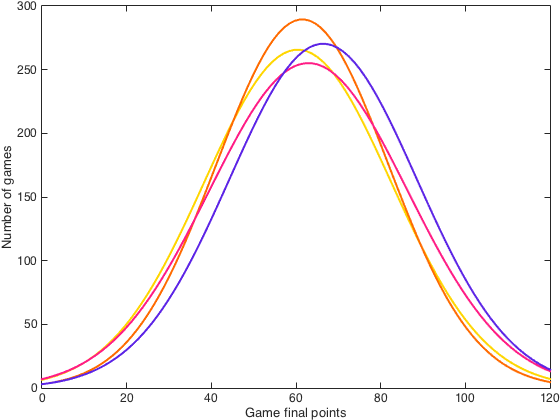
\includegraphics[width=0.5\textwidth]{./img/4/DEFG}
  \caption{filipa}
\label{fig:DEFG}
\end{figure}

Figure~\ref{fig:DEFG} presents the Gaussian fitting curves of the scenarios (d) and (e) as reference points, and scenarios (f) and (g).
The final points obtained by the team with 1 Deep-1 player and 1 Rule-based (f, pink) were higher than the ones obtained by the team with 1 Trick and 1 Rule-based (d, yellow), which is visible in the density between 80 and 120 points.
Similarly, the team with 2 Deep-1 players also has its Gaussian fitting curve on the right of the team with 2 Trick players, suggesting its achieved final points were higher.

\begin{figure}[h]
        \centering
        \begin{subfigure}[h]{0.32\textwidth}
                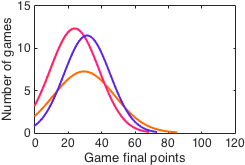
\includegraphics[width=\textwidth]{./img/4/DEFGhard}
                \caption{filipa}
                \label{fig:DEFGhard}
        \end{subfigure}
        \begin{subfigure}[h]{0.32\textwidth}
                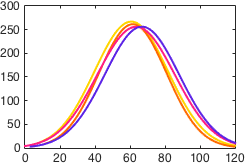
\includegraphics[width=\textwidth]{./img/4/DEFGmedium}
                \caption{filipa}
                \label{fig:DEFGmedium}
        \end{subfigure}
        \begin{subfigure}[h]{0.32\textwidth}
                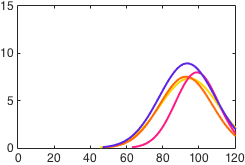
\includegraphics[width=\textwidth]{./img/4/DEFGeasy}
                \caption{filipa}
                \label{fig:DEFGeasy}
        \end{subfigure}
        \caption{filipa}
        \label{fig:DEFG-CH}
\end{figure}

Figure~\ref{fig:DEFG-CH} presents the Gaussian fitting curves of scenarios (d), (e), (f) and (g) divided by the three initial hands conditions.
By comparing results of \emph{medium} initial conditions, from scenarios (d) to (g), each evaluated team incrementally improves the previous one.
On the other hand, both teams from scenarios (f) and (g) underperform in the achieved final scores for \emph{hard} initial hands and outperform the achieved finals cores for \emph{easy} initial hands when compared to scenarios (d) and (e).

\begin{figure}[h!]
  \centering
    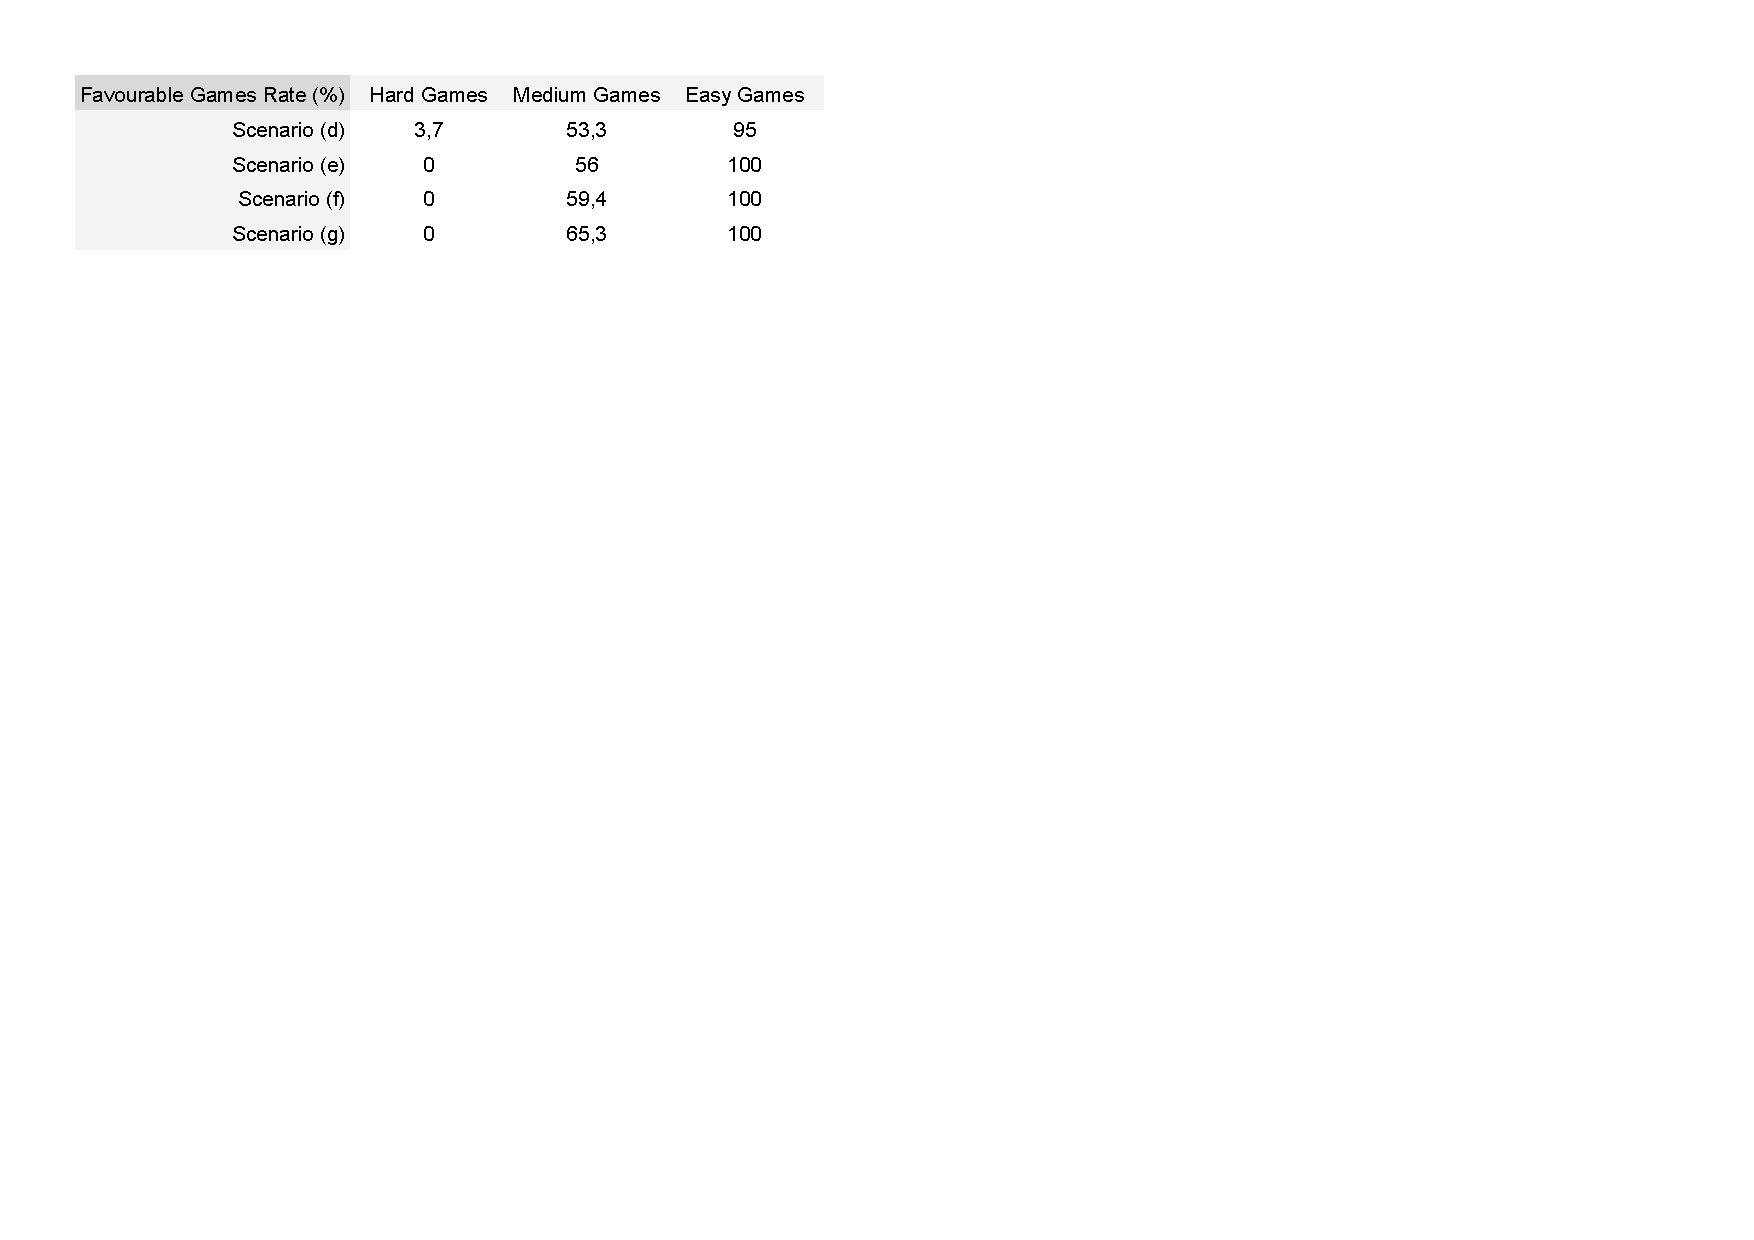
\includegraphics[width=0.7\textwidth]{./img/4/DEFG-fgr}
  \caption{filipa}
\label{fig:DEFG-fgr}
\end{figure}

Finally, the last Figure~\ref{fig:DEFG-fgr} comparing the Deep-1 player and the Trick player agrees with previous conclusions and emphasises the effective competing results of Deep-1 player.


\subsection{The Deep-2 Player}

The last configuration of the \ac{pimc} algorithm is the Deep-2 player.
Its difference from the Deep-1 player is the utility function, modelled by Equation~\ref{eq:uf2}.

\begin{equation} \label{eq:uf2}
u_2 = \left\{
                \begin{array}{ll}
                  2, & teamPoints > 90\\
                  1, & teamPoints > 60\\
                  0.1, & teamPoints > 30\\
                  -2, & opponentTeamPoints >90\\
                  -1, & opponentTeamPoints > 60\\
                  -0.1, & opponentTeamPoints > 30\\
                \end{array}
              \right.
\end{equation}

Instead of maximizing the final points, this utility function groups the final points into 6 possible rewards for the agent and tries to maximize the number of won games.
The main advantage of this utility function is the time spent on the game search, since there are more nodes with the same rewards, and therefore some $\alpha\beta$-cuts occur earlier.
On the other hand, when limiting the depth of the search, without any heuristic, \ac{pimc} algorithm may be misled to worse nodes.

In order to observe the Deep-2 player performance, the following scenarios will be considered:
\begin{itemize}
\item (h) 1000 games with 1 Deep-2 player and 3 Rule-based players [light blue];
\item (i) 1000 games with 2 Deep-2 players against 2 Rule-based players [light green].
\end{itemize}

The overall \ac{fgr} of the team with 1 Deep-2 player and 1 Rule-based (d) was 58.6\% (57.3\% won games and 1.3\% drawn games), and at the same time, the \ac{fgr} of the team with 2 Deep-1 players (e) was 62.6\% (61.79\% won games and 0.7\% drawn games).
In the same way there was a difference between scenarios (f) and (g), having two Deep-2 players on the same team significantly improves the results when compared to only one, although \acp{fgr} have decreased from the last scenarios.

\begin{figure}[h]
        \centering
        \begin{subfigure}[h]{0.4\textwidth}
                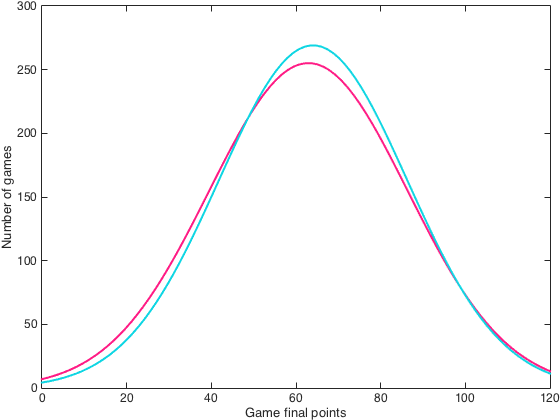
\includegraphics[width=\textwidth]{./img/4/FH}
                \caption{filipa}
                \label{fig:FH}
        \end{subfigure}
        \begin{subfigure}[h]{0.4\textwidth}
                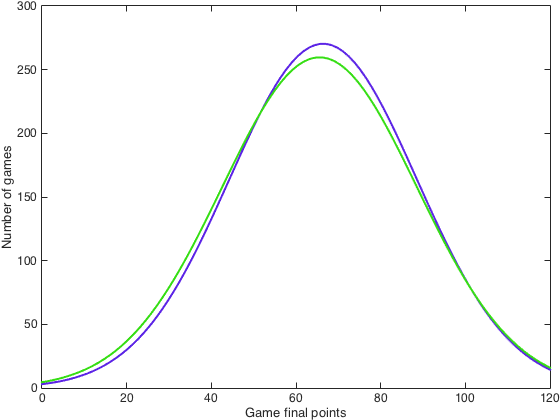
\includegraphics[width=\textwidth]{./img/4/GI}
                \caption{filipa}
                \label{fig:GI}
        \end{subfigure}
        \caption{filipa}
        \label{fig:FGHI}
\end{figure}

Figure~\ref{fig:FH} presents the Gaussian fitting curves of scenario (h) compared to scenario (f), at the same time Figure~\ref{fig:GI} presents the Gaussian fitting curves of scenario (i) compared to scenario (g).
The two main considerations about these charts are the modal values of scenario (g, light blue) in the frontier of winning results; also, the team with 2 Deep-2 players underperforms in the obtained points of the team with 2 Deep-1 players.

\begin{figure}[h]
        \centering
        \begin{subfigure}[h]{0.32\textwidth}
                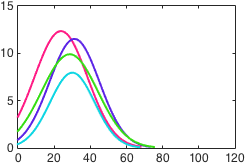
\includegraphics[width=\textwidth]{./img/4/FGHIhard}
                \caption{filipa}
                \label{fig:FGHIhard}
        \end{subfigure}
        \begin{subfigure}[h]{0.32\textwidth}
                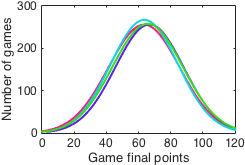
\includegraphics[width=\textwidth]{./img/4/FGHImedium}
                \caption{filipa}
                \label{fig:FGHImedium}
        \end{subfigure}
        \begin{subfigure}[h]{0.32\textwidth}
                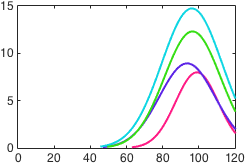
\includegraphics[width=\textwidth]{./img/4/FGHIeasy}
                \caption{filipa}
                \label{fig:FGHIeasy}
        \end{subfigure}
        \caption{filipa}
        \label{fig:FGHI-CH}
\end{figure}

Figure~\ref{fig:FGHI-CH}, as shown for other scenarios, divides the histogram fitting curves of final points into the classifications of the initial conditions.
Slight deviations with the \emph{hard} and \emph{easy} initial conditions are negligible, due to the discrepancy of samples in each scenario.
The \emph{medium} initial conditions chart evidences the similarities in the four approaches.

\begin{figure}[h!]
  \centering
    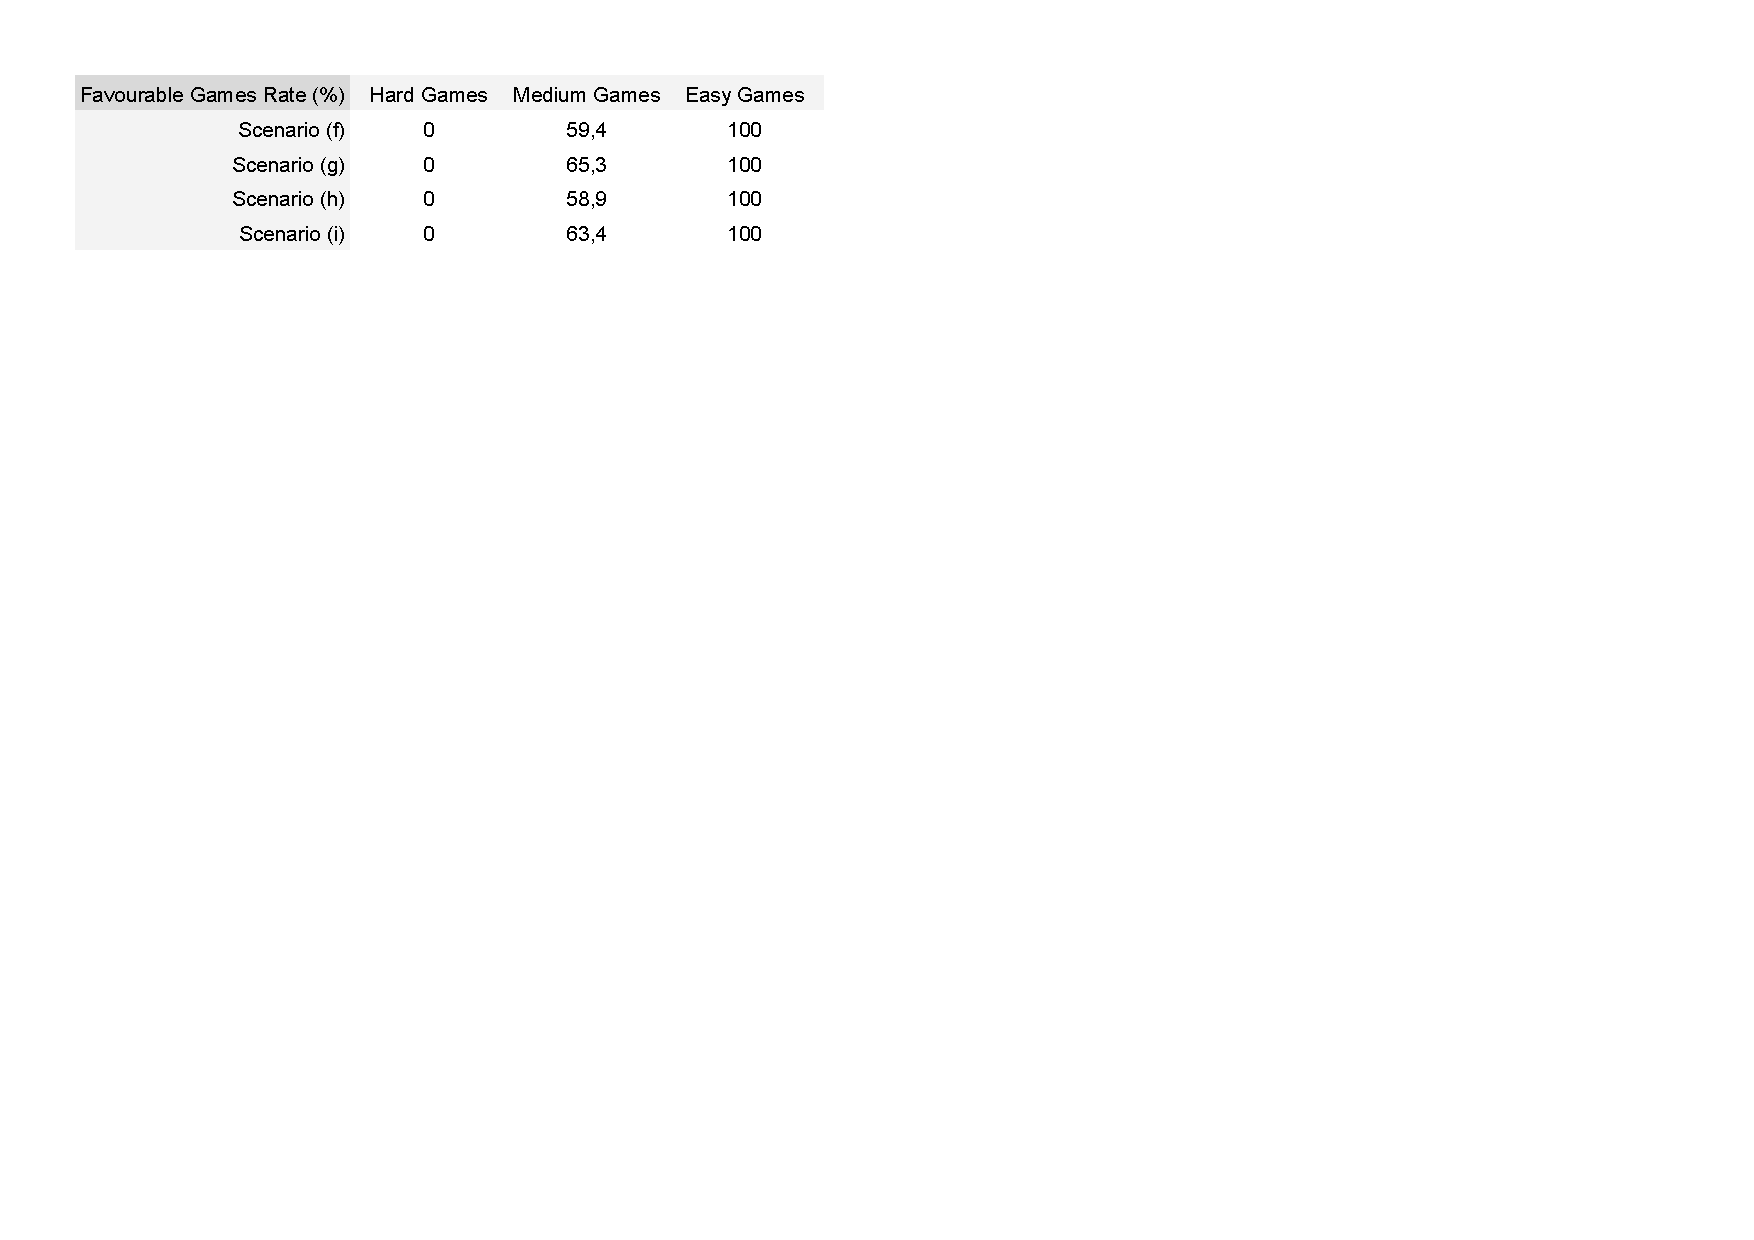
\includegraphics[width=0.7\textwidth]{./img/4/FGHI-fgr}
  \caption{filipa}
\label{fig:FGHI-fgr}
\end{figure}

Additionally, Figure~\ref{FGHI-fgr} presents the \acp{fgr} of scenarios (f), (g), (h) and (i), suggesting that the Deep-2 player underperforms the Deep-1 player.

\subsection{Conclusion}

In order to clearly compare both developed parametrizations of \ac{pimc} algorithm, Figure~\ref{fig:DFH-fgr} summarizes the \ac{fgr} achieved by each player when playing with and against Rule-based players.
Taking the results into account, Deep-1 was the chosen player to participate in the user studies described in Chapter~\ref{chapter:results}.

\begin{figure}[h!]
  \centering
    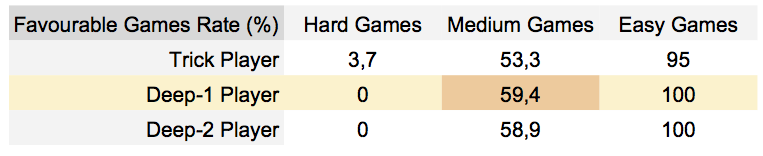
\includegraphics[width=0.7\textwidth]{./img/4/DFH-fgr}
  \caption{filipa}
\label{fig:DFH-fgr}
\end{figure}
